\section{線段樹優化建圖}

\begin{frame}{\ebtitle}
    \begin{problem}[Legacy,Codeforces 786B]
        給定一張 $N$ 個點的有向圖,接下來有 $Q$ 次加邊的操作,每次操作會是以下三種中的一種:
        \begin{itemize}
            \item $1\;v\;u\;w$:從 $v$ 到 $u$ 建一條權重為 $w$ 的邊。
            \item $2\;v\;l\;r\;w$:從 $v$ 到 $[l,r]$ 區間內所有點分別都建一條權重為 $w$ 的邊。
            \item $3\;v\;l\;r\;w$:從 $[l,r]$ 區間內所有點到 $v$ 分別都建一條權重為 $w$ 的邊。
        \end{itemize}
        請你輸出給定的源點 $s$ 到所有點的最短路徑長。
        \begin{itemize}
            \item $1 \le N,Q \le 10^5$。
        \end{itemize}
    \end{problem}
\end{frame}

\begin{frame}{\ebtitle}
    怎麼看起來跟線段樹沒什麼關係

    不急著砸是好事,我們先遺忘世界上所有資料結構
\end{frame}

\begin{frame}{\ebtitle}
    如果每次詢問都是「一個點對所有點,分別都建一條權重為 $w$ 的邊」要怎麼辦?

    \begin{figure}[h!]
        \begin{center}
            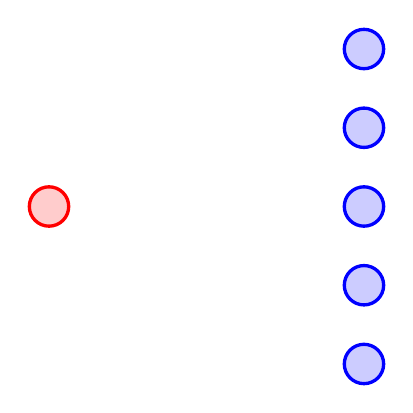
\begin{tikzpicture}[rotate=90, every node/.style={draw, very thick, circle, minimum width=0.5cm}]
                \node[red, fill=red!20!white] at (3, 0) (nd0) {};
                \foreach \i in {1,2,3,4,5} {
                    \node[blue, fill=blue!20!white] at (\i, -4) (nd1-\i) {};
                }
            \end{tikzpicture}
        \end{center}
    \end{figure}
\end{frame}

\begin{frame}{\btitle{「代理人」}}
    \only<1> {
        \begin{figure}[h!]
            \begin{center}
                \begin{tikzpicture}[rotate=90, every node/.style={draw, very thick, circle, minimum width=0.5cm}]
                    \node[red, fill=red!20!white] at (3, 0) (nd0) {};
                    \foreach \i in {1,2,3,4,5} {
                        \node[blue, fill=blue!20!white] at (\i, -4) (nd1-\i) {};
                        \draw[->, very thick, >={Stealth}, red] (nd0) -- (nd1-\i);
                    }
                    \draw[draw=none] (nd0) -- node[red, draw=none, midway, anchor=north east]{$w$} (nd1-1);
                \end{tikzpicture}
            \end{center}
        \end{figure}
    
        注意到,建出來每一條邊都長得一模一樣
    }

    \only<2> {
        \begin{figure}[h!]
            \begin{center}
                \begin{tikzpicture}[rotate=90, every node/.style={draw, very thick, circle, minimum width=0.5cm}]
                    \node[red, fill=red!20!white] at (0, 0) (nd0-1) {};
                    \node[red, fill=red!20!white] at (3, 0) (nd0-2) {};
                    \node[red, fill=red!20!white] at (6, 0) (nd0-3) {};
                    \foreach \i in {1,2,3,4,5} {
                        \node[blue, fill=blue!20!white] at (\i, -4) (nd1-\i) {};
                        \draw[->, very thick, >={Stealth}, red] (nd0-1) -- (nd1-\i);
                        \draw[->, very thick, >={Stealth}, red] (nd0-2) -- (nd1-\i);
                        \draw[->, very thick, >={Stealth}, red] (nd0-3) -- (nd1-\i);
                    }
                \end{tikzpicture}
            \end{center}
        \end{figure}
    }
    
    \only<3> {
        一次詢問建出太多邊了

        \begin{figure}[h!]
            \begin{center}
                \begin{tikzpicture}[rotate=90, every node/.style={draw, very thick, circle, minimum width=0.5cm}]
                    \node[red, fill=red!20!white] at (3, 0) (nd0) {};
                    \node[blue, fill=cyan!50!white] at (3, -3) (nd2) {};
                    \foreach \i in {1,2,3,4,5} {
                        \node[blue, fill=blue!20!white] at (\i, -4) (nd1-\i) {};
                        \draw[->, very thick, >={Stealth}, blue] (nd2) -- (nd1-\i);
                    }
                    \draw[->, very thick, >={Stealth}, red] (nd0) -- node[draw=none, midway, anchor=north east]{$w$} (nd2);
                    \draw[blue, draw=none] (nd2) -- node[draw=none, midway, anchor=north east]{$0$} (nd1-1);
                \end{tikzpicture}
            \end{center}
        \end{figure}
    
        先建一個中間點,中間點再連藍色點\\
        詢問的時候,紅色點連\yum{一條邊}到中間點
    }
    
    \only<4> {
        \begin{figure}[h!]
            \begin{center}
                \begin{tikzpicture}[rotate=90, every node/.style={draw, very thick, circle, minimum width=0.5cm}]
                    \node[red, fill=red!20!white] at (1, 0) (nd0-1) {};
                    \node[red, fill=red!20!white] at (2, 0) (nd0-2) {};
                    \node[red, fill=red!20!white] at (3, 0) (nd0-3) {};
                    \node[red, fill=red!20!white] at (4, 0) (nd0-4) {};
                    \node[red, fill=red!20!white] at (5, 0) (nd0-5) {};
                    \node[blue, fill=cyan!50!white] at (3, -3) (nd2) {};
                    \foreach \i in {1,2,3,4,5} {
                        \node[blue, fill=blue!20!white] at (\i, -4) (nd1-\i) {};
                        \draw[->, very thick, >={Stealth}, blue] (nd2) -- (nd1-\i);
                        \draw[->, very thick, >={Stealth}, red] (nd0-\i) -- (nd2);
                    }
                \end{tikzpicture}
            \end{center}
        \end{figure}
    }

    \only<5> {
        以鬆弛的角度來說,連 $(a, b)$ 邊權 $w$,造成 $d(a) + w \ge d(b)$

        $a$ 連中間人 $c$,$d(a) + w \ge d(c)$ \\
        中間人 $c$ 連 $b_i$,$d(c) + 0 \ge d(b_i)$ \\
        $\Longrightarrow$ 實質上等同 $a$ 連 $b_i$,$d(a) + w \ge d(b_i)$
    }

\end{frame}

\begin{frame}{\ebtitle}
    回到原本的問題,每次詢問要連邊的區間不一樣,每次開新的中間點的話問題沒有半點解決

    如果可以預先決定少少的中間點,每個中間點連到一個區間?\\
    如果可以預先決定一些區間,讓每個詢問都可以被這些區間拆分成少少段?

    \only<2> {
        把中間點開成\yum{線段樹}的樣子
    }
\end{frame}

\begin{frame}{\ebtitle}
    \only<1> {
    \begin{figure}[h!]
        \begin{center}
            \begin{tikzpicture}[
                seg/.style={draw, very thick, rectangle, minimum width=0.5cm, anchor=north west},
                arrow/.style={->, very thick, >={Stealth}, blue},
                bluearr/.style={->, very thick, >={Stealth}, red},
                ndblue/.style={blue, fill={blue!20!white}},
                ndcyan/.style={blue, fill={cyan!50!white}},
                ndwhite/.style={blue, fill={white}},
            ]
                \node[anchor=center, draw, very thick, red, circle, fill=red!20!white] at (-3, -3.4) (nd-qry) {};

                \node[seg, ndwhite, minimum height=5.4cm] (nd-0) at (0, -0.7) {};
                \node[seg, ndwhite, minimum height=2.6cm] (nd-1) at (1, -0.7) {};
                \node[seg, ndwhite, minimum height=1.2cm] (nd-3) at (2, -0.7) {};
                \node[seg, ndblue, minimum height=0.5cm] (nd-7) at (3, -0.7) {1};
                \node[seg, ndblue, minimum height=0.5cm] (nd-8) at (3, -1.4) {2};
                \node[seg, ndwhite, minimum height=1.2cm] (nd-4) at (2, -2.1) {};
                \node[seg, ndblue, minimum height=0.5cm] (nd-9) at (3, -2.1) {3};
                \node[seg, ndblue, minimum height=0.5cm] (nd-10) at (3, -2.8) {4};
                \node[seg, ndwhite, minimum height=2.6cm] (nd-2) at (1, -3.5) {};
                \node[seg, ndwhite, minimum height=1.2cm] (nd-5) at (2, -3.5) {};
                \node[seg, ndblue, minimum height=0.5cm] (nd-11) at (3, -3.5) {5};
                \node[seg, ndblue, minimum height=0.5cm] (nd-12) at (3, -4.2) {6};
                \node[seg, ndwhite, minimum height=1.2cm] (nd-6) at (2, -4.9) {};
                \node[seg, ndblue, minimum height=0.5cm] (nd-13) at (3, -4.9) {7};
                \node[seg, ndblue, minimum height=0.5cm] (nd-14) at (3, -5.6) {8};
                \draw[arrow, blue] (nd-3) -- (nd-7);
                \draw[arrow, blue] (nd-3) -- (nd-8);
                \draw[arrow, blue] (nd-4) -- (nd-9);
                \draw[arrow, blue] (nd-4) -- (nd-10);
                \draw[arrow, blue] (nd-1) -- (nd-3);
                \draw[arrow, blue] (nd-1) -- (nd-4);
                \draw[arrow, blue] (nd-5) -- (nd-11);
                \draw[arrow, blue] (nd-5) -- (nd-12);
                \draw[arrow, blue] (nd-6) -- (nd-13);
                \draw[arrow, blue] (nd-6) -- (nd-14);
                \draw[arrow, blue] (nd-2) -- (nd-5);
                \draw[arrow, blue] (nd-2) -- (nd-6);
                \draw[arrow, blue] (nd-0) -- (nd-1);
                \draw[arrow, blue] (nd-0) -- (nd-2);
            \end{tikzpicture}
        \end{center}
    \end{figure}
    }

    \only<2> {
    \begin{figure}[h!]
        \begin{center}
            \begin{tikzpicture}[
                seg/.style={draw, very thick, rectangle, minimum width=0.5cm, anchor=north west},
                arrow/.style={->, very thick, >={Stealth}, blue},
                bluearr/.style={->, very thick, >={Stealth}, red},
                ndblue/.style={blue, fill={blue!20!white}},
                ndcyan/.style={blue, fill={cyan!50!white}},
                ndwhite/.style={blue, fill={white}},
                ndgray/.style={gray, fill={white}},
            ]
                \node[seg, ndgray, minimum height=5.4cm] (nd-0) at (0, -0.7) {};\node[seg, ndgray, minimum height=2.6cm] (nd-1) at (1, -0.7) {};\node[seg, ndgray, minimum height=1.2cm] (nd-3) at (2, -0.7) {};\node[seg, ndgray, minimum height=0.5cm] (nd-7) at (3, -0.7) {1};\node[seg, ndgray, minimum height=0.5cm] (nd-8) at (3, -1.4) {2};\node[seg, ndwhite, minimum height=1.2cm] (nd-4) at (2, -2.1) {};\node[seg, ndblue, minimum height=0.5cm] (nd-9) at (3, -2.1) {3};\node[seg, ndblue, minimum height=0.5cm] (nd-10) at (3, -2.8) {4};\node[seg, ndwhite, minimum height=2.6cm] (nd-2) at (1, -3.5) {};\node[seg, ndwhite, minimum height=1.2cm] (nd-5) at (2, -3.5) {};\node[seg, ndblue, minimum height=0.5cm] (nd-11) at (3, -3.5) {5};\node[seg, ndblue, minimum height=0.5cm] (nd-12) at (3, -4.2) {6};\node[seg, ndwhite, minimum height=1.2cm] (nd-6) at (2, -4.9) {};\node[seg, ndblue, minimum height=0.5cm] (nd-13) at (3, -4.9) {7};\node[seg, ndblue, minimum height=0.5cm] (nd-14) at (3, -5.6) {8};
                \draw[arrow, gray] (nd-3) -- (nd-7);\draw[arrow, gray] (nd-3) -- (nd-8);\draw[arrow, blue] (nd-4) -- (nd-9);\draw[arrow, blue] (nd-4) -- (nd-10);\draw[arrow, gray] (nd-1) -- (nd-3);\draw[arrow, gray] (nd-1) -- (nd-4);\draw[arrow, blue] (nd-5) -- (nd-11);\draw[arrow, blue] (nd-5) -- (nd-12);\draw[arrow, blue] (nd-6) -- (nd-13);\draw[arrow, blue] (nd-6) -- (nd-14);\draw[arrow, blue] (nd-2) -- (nd-5);\draw[arrow, blue] (nd-2) -- (nd-6);\draw[arrow, gray] (nd-0) -- (nd-1);\draw[arrow, gray] (nd-0) -- (nd-2);

                \node[anchor=center, draw, very thick, red, circle, fill=red!20!white] at (-3, -3.4) (nd-qry) {};
                \draw[arrow, red] (nd-qry) -- (nd-2);
                \draw[arrow, red] (nd-qry) -- (nd-4);
                \node[left of=nd-qry] {$[3, 8]$};
            \end{tikzpicture}
        \end{center}
    \end{figure}
    }

    \only<3> {
    \begin{figure}[h!]
        \begin{center}
            \begin{tikzpicture}[
                seg/.style={draw, very thick, rectangle, minimum width=0.5cm, anchor=north west},
                arrow/.style={->, very thick, >={Stealth}, blue},
                bluearr/.style={->, very thick, >={Stealth}, red},
                ndblue/.style={blue, fill={blue!20!white}},
                ndcyan/.style={blue, fill={cyan!50!white}},
                ndwhite/.style={blue, fill={white}},
                ndgray/.style={gray, fill={white}},
            ]
                \node[seg, ndgray, minimum height=5.4cm] (nd-0) at (0, -0.7) {};\node[seg, ndgray, minimum height=2.6cm] (nd-1) at (1, -0.7) {};\node[seg, ndgray, minimum height=1.2cm] (nd-3) at (2, -0.7) {};\node[seg, ndgray, minimum height=0.5cm] (nd-7) at (3, -0.7) {1};\node[seg, ndblue, minimum height=0.5cm] (nd-8) at (3, -1.4) {2};\node[seg, ndwhite, minimum height=1.2cm] (nd-4) at (2, -2.1) {};\node[seg, ndblue, minimum height=0.5cm] (nd-9) at (3, -2.1) {3};\node[seg, ndblue, minimum height=0.5cm] (nd-10) at (3, -2.8) {4};\node[seg, ndwhite, minimum height=2.6cm] (nd-2) at (1, -3.5) {};\node[seg, ndwhite, minimum height=1.2cm] (nd-5) at (2, -3.5) {};\node[seg, ndblue, minimum height=0.5cm] (nd-11) at (3, -3.5) {5};\node[seg, ndblue, minimum height=0.5cm] (nd-12) at (3, -4.2) {6};\node[seg, ndwhite, minimum height=1.2cm] (nd-6) at (2, -4.9) {};\node[seg, ndblue, minimum height=0.5cm] (nd-13) at (3, -4.9) {7};\node[seg, ndblue, minimum height=0.5cm] (nd-14) at (3, -5.6) {8};
                \draw[arrow, gray] (nd-3) -- (nd-7);\draw[arrow, gray] (nd-3) -- (nd-8);\draw[arrow, blue] (nd-4) -- (nd-9);\draw[arrow, blue] (nd-4) -- (nd-10);\draw[arrow, gray] (nd-1) -- (nd-3);\draw[arrow, gray] (nd-1) -- (nd-4);\draw[arrow, blue] (nd-5) -- (nd-11);\draw[arrow, blue] (nd-5) -- (nd-12);\draw[arrow, blue] (nd-6) -- (nd-13);\draw[arrow, blue] (nd-6) -- (nd-14);\draw[arrow, blue] (nd-2) -- (nd-5);\draw[arrow, blue] (nd-2) -- (nd-6);\draw[arrow, gray] (nd-0) -- (nd-1);\draw[arrow, gray] (nd-0) -- (nd-2);

                \node[anchor=center, draw, very thick, red, circle, fill=red!20!white] at (-3, -3.4) (nd-qry-1) {};
                \draw[arrow, red] (nd-qry-1) -- (nd-2);
                \draw[arrow, red] (nd-qry-1) -- (nd-4);
                \node[left of=nd-qry-1] {$[3, 8]$};
                
                \node[anchor=center, draw, very thick, red, circle, fill=red!20!white] at (-3, -1.4) (nd-qry-2) {};
                \draw[arrow, red] (nd-qry-2) -- (nd-4);
                \draw[arrow, red] (nd-qry-2) -- (nd-8);
                \node[left of=nd-qry-2] {$[2, 4]$};
                
                \node[anchor=center, draw, very thick, red, circle, fill=red!20!white] at (-3, -5.4) (nd-qry-3) {};
                \draw[arrow, red] (nd-qry-3) -- (nd-13);
                \node[left of=nd-qry-3] {$[7, 7]$};
                
            \end{tikzpicture}
        \end{center}
    \end{figure}
    }
\end{frame}

\begin{frame}{\ebtitle}
    對一個線段樹節點連一條邊,等同於對區間內所有點分別連邊
    
    如果把整張圖反過來:從線段樹節點連出來,等同於從區間內所有點分別連出來
\end{frame}

\begin{frame}{\ebtitle}
    \begin{figure}[h!]
        \begin{center}
            \begin{tikzpicture}[
                seg/.style={draw, very thick, rectangle, minimum width=0.5cm, anchor=north west},
                arrow/.style={->, very thick, >={Stealth}, blue},
                bluearr/.style={->, very thick, >={Stealth}, red},
                ndblue/.style={blue, fill={blue!20!white}},
                ndcyan/.style={blue, fill={cyan!50!white}},
                ndwhite/.style={blue, fill={white}},
                ndgray/.style={gray, fill={white}},
            ]
                \node[seg, ndgray, minimum height=5.4cm] (nd-0) at (0, -0.7) {};\node[seg, ndgray, minimum height=2.6cm] (nd-1) at (1, -0.7) {};\node[seg, ndgray, minimum height=1.2cm] (nd-3) at (2, -0.7) {};\node[seg, ndgray, minimum height=0.5cm] (nd-7) at (3, -0.7) {1};\node[seg, ndblue, minimum height=0.5cm] (nd-8) at (3, -1.4) {2};\node[seg, ndwhite, minimum height=1.2cm] (nd-4) at (2, -2.1) {};\node[seg, ndblue, minimum height=0.5cm] (nd-9) at (3, -2.1) {3};\node[seg, ndblue, minimum height=0.5cm] (nd-10) at (3, -2.8) {4};\node[seg, ndwhite, minimum height=2.6cm] (nd-2) at (1, -3.5) {};\node[seg, ndwhite, minimum height=1.2cm] (nd-5) at (2, -3.5) {};\node[seg, ndblue, minimum height=0.5cm] (nd-11) at (3, -3.5) {5};\node[seg, ndblue, minimum height=0.5cm] (nd-12) at (3, -4.2) {6};\node[seg, ndwhite, minimum height=1.2cm] (nd-6) at (2, -4.9) {};\node[seg, ndblue, minimum height=0.5cm] (nd-13) at (3, -4.9) {7};\node[seg, ndblue, minimum height=0.5cm] (nd-14) at (3, -5.6) {8};
                \draw[arrow, gray] (nd-7) -- (nd-3);\draw[arrow, gray] (nd-8) -- (nd-3);\draw[arrow, blue] (nd-9) -- (nd-4);\draw[arrow, blue] (nd-10) -- (nd-4);\draw[arrow, gray] (nd-3) -- (nd-1);\draw[arrow, gray] (nd-4) -- (nd-1);\draw[arrow, blue] (nd-11) -- (nd-5);\draw[arrow, blue] (nd-12) -- (nd-5);\draw[arrow, blue] (nd-13) -- (nd-6);\draw[arrow, blue] (nd-14) -- (nd-6);\draw[arrow, blue] (nd-5) -- (nd-2);\draw[arrow, blue] (nd-6) -- (nd-2);\draw[arrow, gray] (nd-1) -- (nd-0);\draw[arrow, gray] (nd-2) -- (nd-0);
                
                \node[anchor=center, draw, very thick, red, circle, fill=red!20!white] at (-3, -3.4) (nd-qry-1) {};
                \draw[arrow, red] (nd-2) -- (nd-qry-1);
                \draw[arrow, red] (nd-4) -- (nd-qry-1);
                \node[left of=nd-qry-1] {$[3, 8]$};
                
                \node[anchor=center, draw, very thick, red, circle, fill=red!20!white] at (-3, -1.4) (nd-qry-2) {};
                \draw[arrow, red] (nd-4) -- (nd-qry-2);
                \draw[arrow, red] (nd-8) -- (nd-qry-2);
                \node[left of=nd-qry-2] {$[2, 4]$};
                
                \node[anchor=center, draw, very thick, red, circle, fill=red!20!white] at (-3, -5.4) (nd-qry-3) {};
                \draw[arrow, red] (nd-13) -- (nd-qry-3);
                \node[left of=nd-qry-3] {$[7, 7]$};
                
            \end{tikzpicture}
        \end{center}
    \end{figure}
\end{frame}

\begin{frame}{\ebtitle}
    預先建兩棵線段樹,一棵從根往葉子連邊,一棵從葉子往根連邊 \\
    每次詢問根據方向在對應的樹上連 $O(\log N)$ 條邊,就可以建出一樣的圖(在最短路的意義上一樣)

    單源最短路?dijkstra 就好
\end{frame}

\begin{frame}{\ebtitle}
    最後建出來的圖上:
    \begin{itemize}
        \item 一棵線段樹有 $2N$ 個節點,但是兩棵線段樹葉節點可以共用,總共 $3N$ 個點
        \item 兩棵線段樹各建 $O(N)$ 條邊,之後每個詢問建 $O(\log N)$ 條邊,總共 $O(N + Q \log N)$ 條邊
    \end{itemize}
    時間複雜度 $O((N + Q \log N) \log N)$
\end{frame}

\begin{frame}{\ebtitle}
    線段樹本身和我們是怎麼建圖的並\yum{沒有}關係 \\
    我們甚至可以用 sparse table 建類似的圖

    線段樹在這裡發揮的最大價值是\yum{把詢問區間拆解}成一些特別的小區間
\end{frame}
